\section{Some useful results}

\begin{lemma}
  Let $\Gamma$ be a transitive sggi over $n$ points such that the CPR graph have exactly $n-1$ edges. Then the CPR graph of $\Gamma$ is a string.
\end{lemma}

\begin{proof}\label{graphIsString}
  $\Gamma$ is transitive so its CPR graph is connected. And, because we have $n-1$ edges for $n$ vertices, the graph must be a tree.

  \paragraph{}
  Suppose now, that we have a vertex with at least three edges. Those edges are labelled with three differents numbers, $i, j, k$ that describe three different involutions, $\rho_i, \rho_j$ and $\rho_k$. But at least two of those involutions are not adjacent and so must commute. We will consider that the involution $\rho_i$ and $\rho_k$ does commute.

  \paragraph{}
  And so by proposition 3.5 of~\cite{cprGraph}, the CPR graph where we only keep edge labelled with $i$ and $k$ must only contains those patterns:
  \begin{itemize}
    \item Fixed points
    \item Isolated edge (labelled with $i$ or $k$)
    \item Double edge
    \item Alternating square
  \end{itemize}
  But in our case, we already have two edges labelled $i$ and $k$ that connect the same point to two differents points. So the only way, we can extend this to a good pattern is with an alternating square. But we cannot have an alternating square because the graph is a tree and thus does not contains cycles.

  \paragraph{}
  So we cannot have vertex with three edges but the graph must be connected, so the only solution is a string.
\end{proof}

\begin{lemma}\label{rho0atEnd}
  Let $\Gamma$ be a sggi with generators $\rho_0, \rho_1, \dots$ such that its CPR graph is a string. If $\rho_0$ and $\rho_1$ are 2-transpositions, then an edge of $\rho_0$ must be placed at an end of the CPR graph.
\end{lemma}

\begin{proof}
  The CPR graph is a string so we cannot have alterning square or double edge, thus two involutions that must commute can not share a vertex. By definition of a sggi, the $\rho_0$ involution must commute with all other involutions except $\rho_1$. The $\rho_0$ edges must only share vertices with $\rho_1$ but there are two edges for each involution. But each $\rho_0$ edge must be surrounded by two $\rho_1$ if it's not at an end of the graph. We can save one $\rho_1$ edge if it's surrounded by two $\rho_0$ edges but even with that we need three $\rho_1$ edges with we are not placing a $\rho_0$ edge at a end of the graph but we only have two of them. Therefore one $\rho_0$ edge is at an end of the graph.
\end{proof}

\begin{lemma}
  Let $\Gamma$ be a sggi avec $A_{11}$. Then $\Gamma$ contains at least two 4-transpositions if it's of rank 4 and at least one 4-transposition if its rank is 5.
\end{lemma}

\begin{proof}
  Suppose that there exists a sggi of rank 5 with only 2-transposition or a sggi of rank 4 with only one 4-transposition. In both case, we have exactly 10 edges for 11 vertices. We can apply the lemma~\ref{graphIsString} and so the CPR graph of $\Gamma$ is a string.

  \paragraph{Rank 5}
  In this case, we have five involutions and all of them are 2-transpositions. We can apply the lemma~\ref{rho0atEnd} and so an $\rho_0$ edge must be at one end of the graph. By duality, we can do the same with $\rho_4$ and so there is an $\rho_4$ edge at the other end.

  \paragraph{}
  Because the other end is occupied, the other edge of $\rho_0$ cannot go there. So a $\rho_1$ edge must be between the two $\rho_0$ edge (see the proof of lemma~\ref{rho0atEnd} for details). We can apply the same reasonning to $\rho_3$ by duality. At this point, we have the following graph

  \begin{figure}[H]
    \begin{center}
      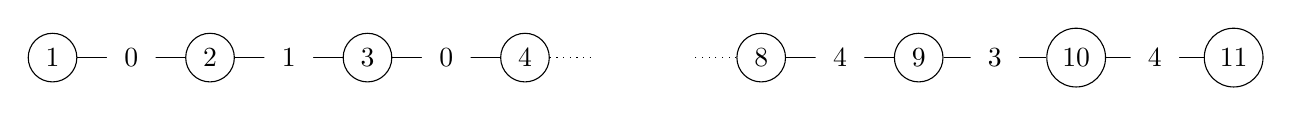
\begin{tikzpicture}

        \begin{scope}[every node/.style={circle,draw}]
          \node (1)  at (0,0)  {1};
          \node (2)  at (2,0)  {2};
          \node (3)  at (4,0)  {3};
          \node (4)  at (6,0)  {4};
          \node (8)  at (9,0)  {8};
          \node (9)  at (11,0) {9};
          \node (10) at (13,0) {10};
          \node (11) at (15,0) {11};
        \end{scope}

        \node (4b) at (7,0) {};
        \node (8b) at (8,0) {};

        \begin{scope}[every node/.style={fill=white,circle}]

          \begin{scope}[every edge/.style={draw}]
            \path (1)  edge node {$0$} (2);
            \path (2)  edge node {$1$} (3);
            \path (3)  edge node {$0$} (4);
            \path (4)  edge[style={dotted}] (4b);
            \path (8)  edge[style={dotted}] (8b);
            \path (8)  edge node {$4$} (9);
            \path (9)  edge node {$3$} (10);
            \path (10) edge node {$4$} (11);
          \end{scope}
        \end{scope}



      \end{tikzpicture}
      \caption{}
    \end{center}
  \end{figure}

  \paragraph{}
  We must connect the $\rho_0$ and $\rho_4$ edges to something but the only possibilities are to use a $\rho_1$ and a $\rho_3$ edge and now we have the following graph and we must still add two $\rho_2$ edges but they will be adjacent and that is forbidden in a CPR graph.

  \begin{figure}[H]
    \begin{center}
      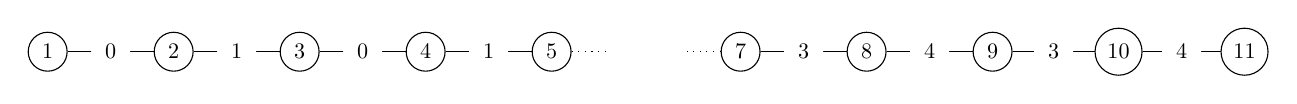
\begin{tikzpicture}[scale=0.8]

        \begin{scope}[every node/.style={circle,draw,transform shape}]
          \node (1)  at (0,0)  {1};
          \node (2)  at (2,0)  {2};
          \node (3)  at (4,0)  {3};
          \node (4)  at (6,0)  {4};
          \node (5)  at (8,0)  {5};
          \node (7)  at (11,0) {7};
          \node (8)  at (13,0) {8};
          \node (9)  at (15,0) {9};
          \node (10) at (17,0) {10};
          \node (11) at (19,0) {11};
        \end{scope}

        \node (5b) at (9,0) {};
        \node (7b) at (10,0) {};

        \begin{scope}[every node/.style={fill=white,circle,transform shape}]

          \begin{scope}[every edge/.style={draw}]
            \path (1)  edge node {$0$} (2);
            \path (2)  edge node {$1$} (3);
            \path (3)  edge node {$0$} (4);
            \path (4)  edge node {$1$} (5);
            \path (5)  edge[style={dotted}] (5b);
            \path (7)  edge[style={dotted}] (7b);
            \path (7)  edge node {$3$} (8);
            \path (8)  edge node {$4$} (9);
            \path (9)  edge node {$3$} (10);
            \path (10) edge node {$4$} (11);
          \end{scope}
        \end{scope}



      \end{tikzpicture}
      \caption{}
    \end{center}
  \end{figure}


  \paragraph{Rank 4}
  We have exactly one 4-transposition. We have two cases: $\rho_0$ is a 4-transposition or $\rho_1$. If $\rho_0$ is a 4-transposition, then $\rho_1$ is a 2-transposition but all $\rho_0$ must be surrounded by $\rho_1$ involutions but that impossible.

  \paragraph{}
  So $\rho_1$ must be a 4-transposition. Therefore $\rho_3$ and $\rho_2$ are 2-transposition. And so by lemma~\ref{rho0atEnd}, a $\rho_3$ edge must be placed at an end, followed by a $\rho_2$ edge. For the other $\rho_3$ edge, we have two possibilities, it can be placed next to the first one or at the other end.

  \paragraph{}
  In the first case, we have the following graph. But the only way, we can complete it is by using a sequence $\rho_1, \rho_0, \rho_1, \rho_0, \rho_1$ but we still have a $\rho_1$ edge that cannot be placed.

  \begin{figure}[H]
    \begin{center}
      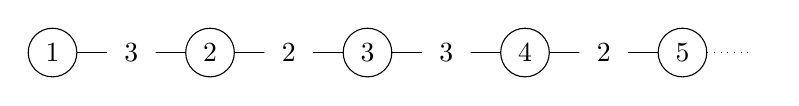
\begin{tikzpicture}

        \begin{scope}[every node/.style={circle,draw}]
          \node (1)  at (0,0)  {1};
          \node (2)  at (2,0)  {2};
          \node (3)  at (4,0)  {3};
          \node (4)  at (6,0)  {4};
          \node (5)  at (8,0)  {5};
        \end{scope}

        \node (6)  at (9,0) {};

        \begin{scope}[every node/.style={fill=white,circle}]

          \begin{scope}[every edge/.style={draw}]
            \path (1)  edge node {$3$} (2);
            \path (2)  edge node {$2$} (3);
            \path (3)  edge node {$3$} (4);
            \path (4)  edge node {$2$} (5);
            \path (5)  edge[style={dotted}] (6);
          \end{scope}
        \end{scope}

      \end{tikzpicture}
      \caption{}
    \end{center}
  \end{figure}

\paragraph{}
For the second case, we have this graph. On each side, we must continue with a sequence $\rho_1, \rho_0, \rho_1$. And we have used every edge but in the middle a point is linked with the $\rho_1$ edge and that is forbidden.

\begin{figure}[H]
  \begin{center}
    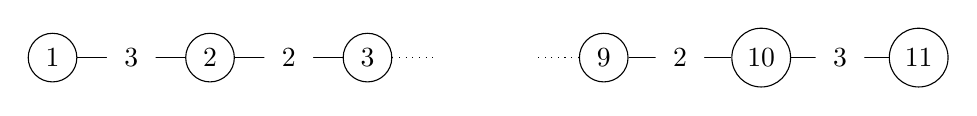
\begin{tikzpicture}

      \begin{scope}[every node/.style={circle,draw}]
        \node (1)  at (0,0)  {1};
        \node (2)  at (2,0)  {2};
        \node (3)  at (4,0)  {3};
        \node (9)  at (7,0)  {9};
        \node (10) at (9,0)  {10};
        \node (11) at (11,0) {11};
      \end{scope}

      \node (3b) at (5,0)  {};
      \node (9b) at (6,0)  {};


      \begin{scope}[every node/.style={fill=white,circle}]

        \begin{scope}[every edge/.style={draw}]
          \path (1)  edge node {$3$} (2);
          \path (2)  edge node {$2$} (3);
          \path (3)  edge[style={dotted}] (3b);
          \path (9)  edge[style={dotted}] (9b);
          \path (9)  edge node {$2$} (10);
          \path (10) edge node {$3$} (11);
        \end{scope}
      \end{scope}

    \end{tikzpicture}
    \caption{}
  \end{center}
\end{figure}

\end{proof}

\begin{lemma}
  For all sggi over $A_{11}$, it's not possible to have two non-adjacent 4-tranpositions if there is no 4-transposition between them.
\end{lemma}

\begin{proof}

Maybe two complicated to prove this in general and it's easier to use it only when we need it.

%  Appelons les deux transpositions en question $\rho_i$ et $\rho_j$. Plaçons $\rho_i$ sur le graphe:

%  \begin{figure}[H]
%    \begin{center}
%      \begin{tikzpicture}

%        \begin{scope}[every node/.style={circle,draw}]
%          \node (1)  at (0,2)  {1};
%          \node (2)  at (0,0)  {2};
%          \node (3)  at (2,2)  {3};
%          \node (4)  at (2,0)  {4};
%          \node (5)  at (4,2)  {5};
%          \node (6)  at (4,0)  {6};
%          \node (7)  at (6,2)  {7};
%          \node (8)  at (6,0)  {8};
%          \node (9)  at (8,2)  {9};
%          \node (10) at (8,0)  {10};
%          \node (11) at (10,2) {11};
%        \end{scope}

%        \begin{scope}[every node/.style={fill=white,circle}]

%          \begin{scope}[every edge/.style={draw}]
%            \path (1)  edge node {$i$} (2);
%            \path (3)  edge node {$i$} (4);
%            \path (5)  edge node {$i$} (6);
%            \path (7)  edge node {$i$} (8);
%          \end{scope}
%        \end{scope}

%      \end{tikzpicture}
%      \caption{Une seule 4-transposition $\rho_i$}
%    \end{center}
%  \end{figure}

%  \paragraph{}
%  Si nous voulons placer les arêtes de $\rho_j$ de telle sorte que $\rho_i$ commute avec $\rho_j$, alors, par la proposition 3.5 de~\cite{cprGraph} on doit utiliser une des trois solutions suivantes:
%  \begin{enumerate}
%    \item Doubler une arête de $\rho_i$
%    \item Former un carré alterné avec $\rho_i$
%    \item Relier deux points fixés par $\rho_i$.
%  \end{enumerate}

%  \paragraph{}
%  Remarquons que le fait de relier deux points fixés par $\rho_i$ ne peut être utilisé que pour placer une des quatre arêtes de $\rho_j$. Donc nous devons trouver une solution pour au moins les trois restantes. Nous avons donc les possibilités suivantes:
%  \begin{enumerate}
%    \item Deux carrés alternés
%    \item Un carré alterné, une arête doublée et une arête reliant des points fixes
%    \item Un carré alterné et deux arête doublées
%    \item Trois arêtes doublées et une arête reliant deux points fixes
%    \item Quatre arêtes doublées.
%  \end{enumerate}

%  \paragraph{}
%  Nous allons traiter les cas un par un

%  \paragraph{Deux carrés alternés}
%  Dessinons le graphe CPR de ce cas

%  \begin{figure}[H]
%    \begin{center}
%      \begin{tikzpicture}

%        \begin{scope}[every node/.style={circle,draw}]
%          \node (1)  at (0,2)  {1};
%          \node (2)  at (0,0)  {2};
%          \node (3)  at (2,2)  {3};
%          \node (4)  at (2,0)  {4};
%          \node (5)  at (4,2)  {5};
%          \node (6)  at (4,0)  {6};
%          \node (7)  at (6,2)  {7};
%          \node (8)  at (6,0)  {8};
%          \node (9)  at (8,2)  {9};
%          \node (10) at (8,0)  {10};
%          \node (11) at (10,2) {11};
%        \end{scope}

%        \begin{scope}[every node/.style={fill=white,circle}]

%          \begin{scope}[every edge/.style={draw}]
%            \path (1)  edge node {$i$} (2);
%            \path (3)  edge node {$i$} (4);
%            \path (5)  edge node {$i$} (6);
%            \path (7)  edge node {$i$} (8);
%            \path (1)  edge node {$j$} (3);
%            \path (2)  edge node {$j$} (4);
%            \path (5)  edge node {$j$} (7);
%            \path (6)  edge node {$j$} (8);
%          \end{scope}
%        \end{scope}

%      \end{tikzpicture}
%      \caption{Deux 4-transpositions formant deux carrés alternés}
%    \end{center}
%  \end{figure}



\end{proof}
